%-------------------------------------------------------
\section{Contexto - Motivación}
%-------------------------------------------------------
%\subsection{Motivación}
\begin{frame}{Ecosistema de dispositivos}{Contexto - Motivación}
%-------------------------------------------------------
    \begin{figure}				
		{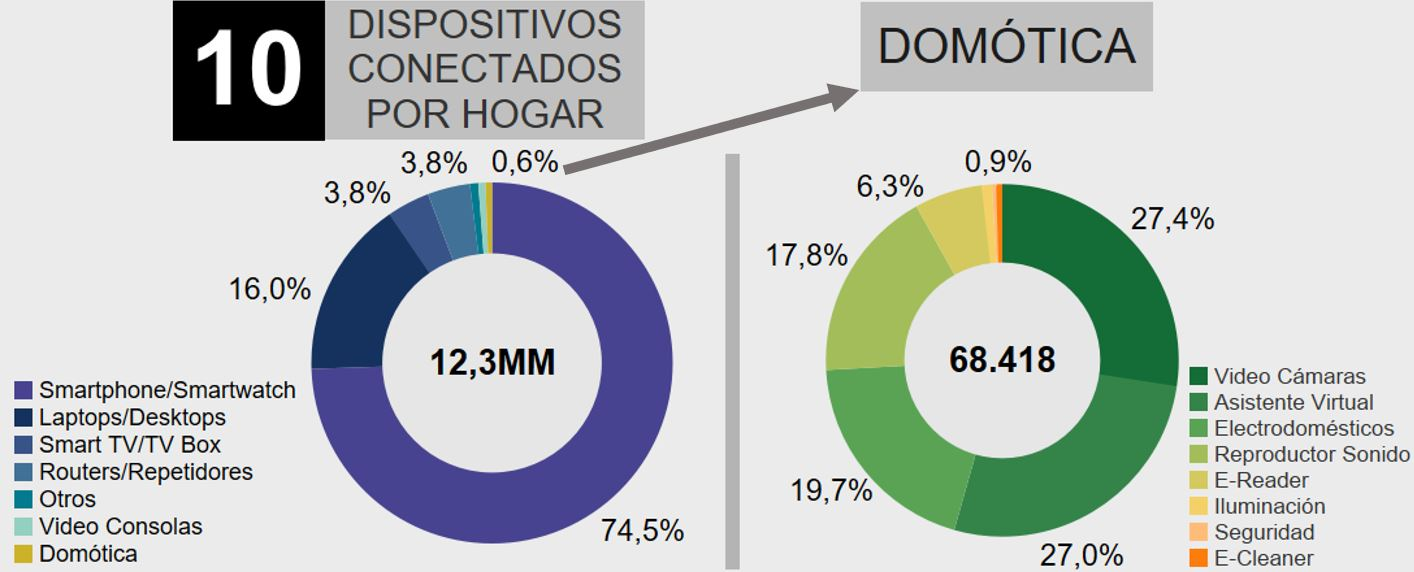
\includegraphics[width=0.99\textwidth,keepaspectratio]{Sustentacion/Figures/DispositivosColombia.JPG}}
		\caption{\small \sl Dispositivos en el mercado colombiano [Fuente Propia]}
		\label{figure:Ecosistema}
    \end{figure}
\end{frame}
%-------------------------------------------------------
\begin{frame}{Comunicaciones M2M}{Contexto - Motivación}
%-------------------------------------------------------
\begin{figure}[htbp]
	    \centering
		\fbox{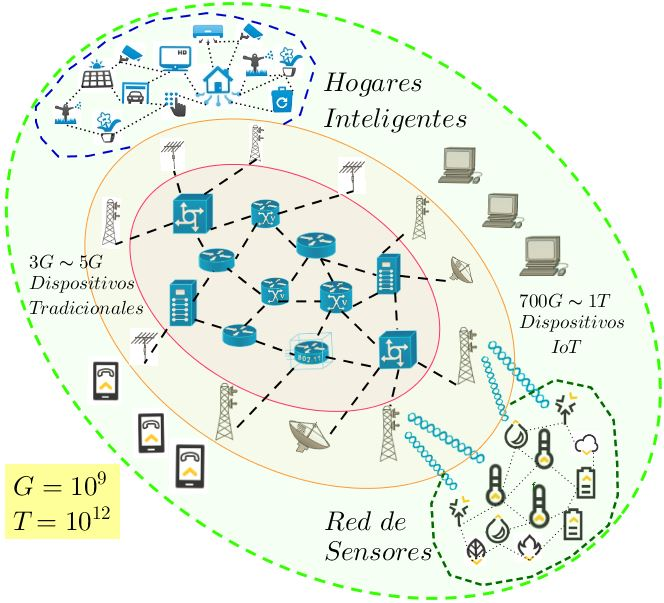
\includegraphics[height=0.7\textheight,keepaspectratio]{Figures/M2M.JPG}}
	    \caption{Comunicaciones M2M \cite{DoWeNeed}}
	    \label{fig:M2M}
    \end{figure}
\end{frame}
%-------------------------------------------------------
\begin{frame}{Paradigma M2M}{Contexto - Motivación}
%-------------------------------------------------------
\begin{block}{Cambio de paradigma}
  \begin{itemize}
    \justifying
    \item<1-|alert@1> Actualmente la industria esta experimentando un crecimiento sin precedentes de sensores y actuadores simples fabricados por diversos proveedores y limitados en recursos computacionales \cite{M2MARCHITECTUREPERFORMANCE}. 
    \item<2-|alert@2> Gestionar y analizar los importantes volúmenes de información, en gran medida redundante, es un reto técnico en las redes actuales \cite{IOTIPV6MIPV6}.
    \item<3-|alert@3> Minimizar los costos acumulados en Hardware/Software, Vigilancia, Gestión y Seguridad es un factor clave en el despliegue del IoT \cite{RethinkIOT}.
    \item<4-|alert@4> No existen arquitecturas de redes de comunicaciones humanas que se adecuen al tamaño del IoT \cite{RethinkIOT}. 
  \end{itemize}
 \end{block}
\end{frame}
%-------------------------------------------------------
%\subsection{Características Generales}
\begin{frame}{Dinámicas de red}{Contexto - Motivación}
%-------------------------------------------------------
    \begin{figure}[htbp]
	    \centering
		\fbox{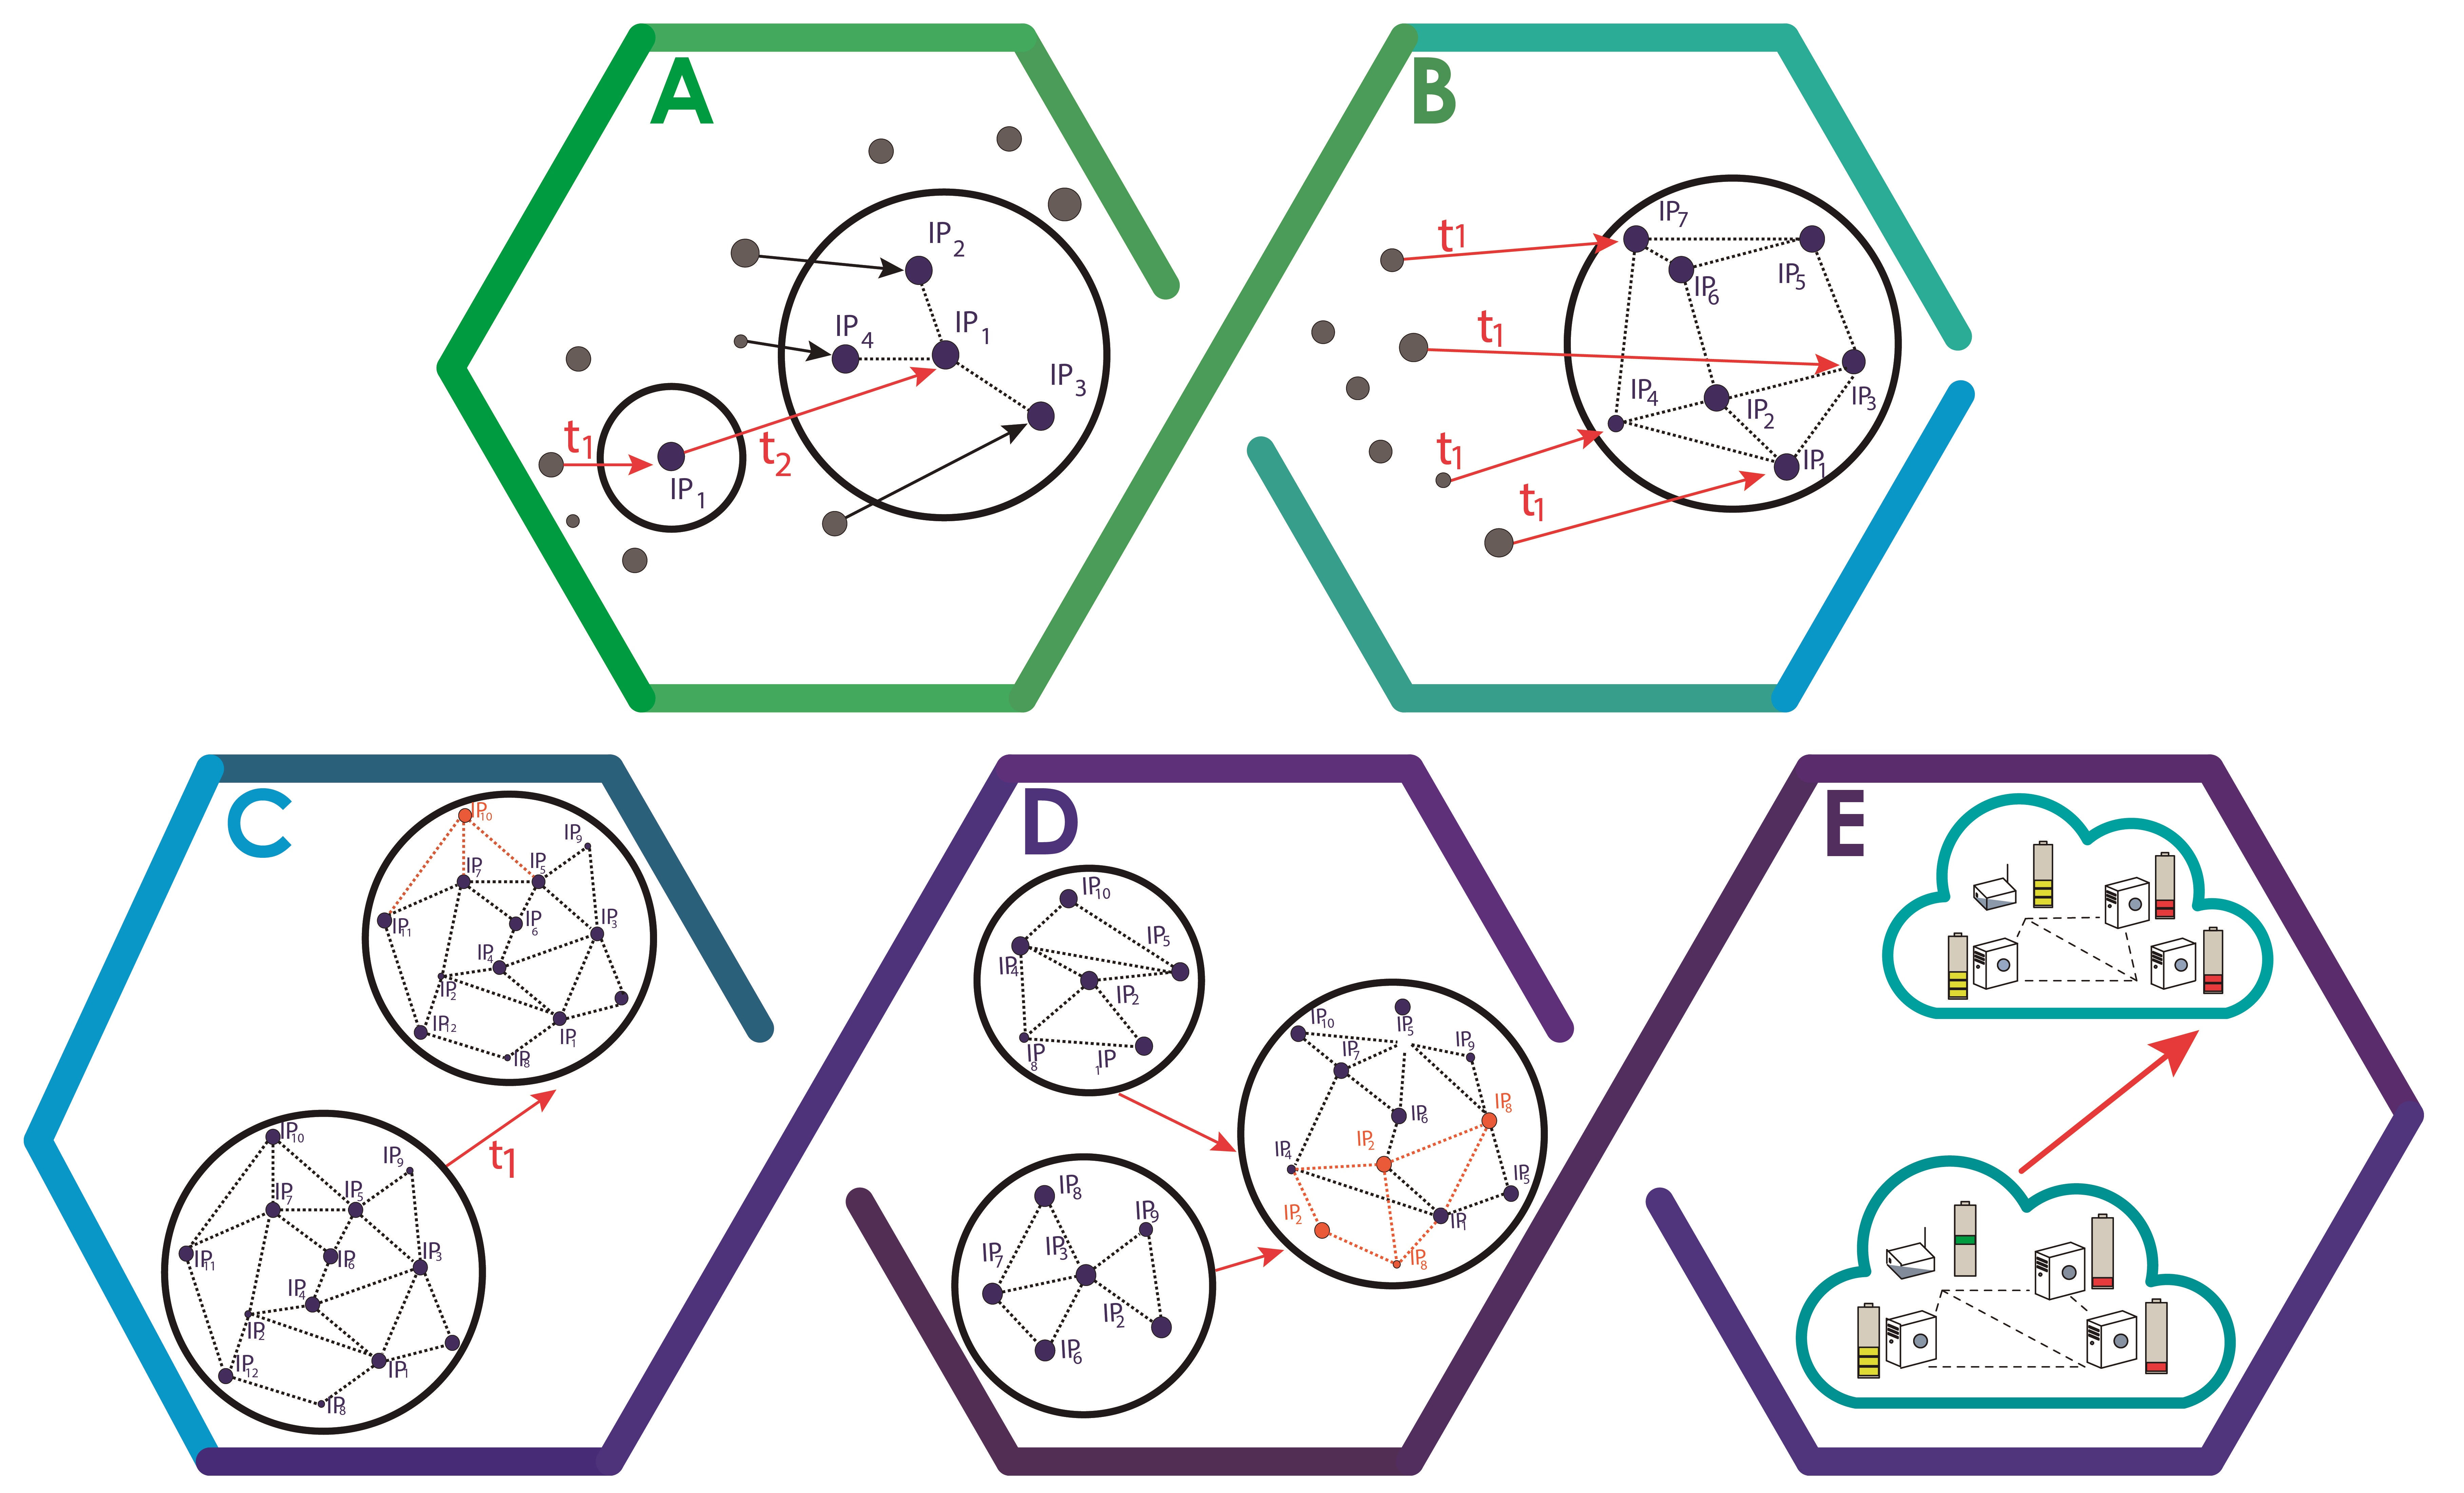
\includegraphics[height=0.65\textheight,keepaspectratio]{Figures/DinamicaManets.jpg}}
	    \caption{Dinámicas de las MANETs [Fuente propia]}
	    \label{fig:DinMan}
    \end{figure}
\end{frame}
%-------------------------------------------------------
%\subsection{Marco Conceptual}
%\begin{frame}{Contexto}{Marco Conceptual \cite{DATMANET}}
%-------------------------------------------------------
%\begin{block}{Requerimientos protocolo de direccionamiento}
%  \begin{itemize}
%    \justifying
%    \item Cada nodo debe obtener una dirección IP dinámicamente.
%    \item En ningún instante del tiempo deberían haber IP's %duplicadas.
%    \item Cuando un nodo ''abandone'' la red, la IP debe ser liberada.
%    \item Cuando se efectué una migración de redes el esquema debe detectar y corregir duplicidades. 
%    \item El protocolo debe asegurar que solo nodos autorizados pueden tener acceso a los recursos. 
%    \item El esquema debe ser tolerante a fallas en los nodos.
%    \item Se deben minimizar los paquetes señalización. 
%  \end{itemize}
% \end{block}
%\end{frame}
